\documentclass[]{article}

\usepackage{mathtools,mathrsfs,url,fancyhdr, graphicx}

\renewcommand{\headrulewidth}{0pt}
\fancyhead[L]{}
\fancyhead[C]{
	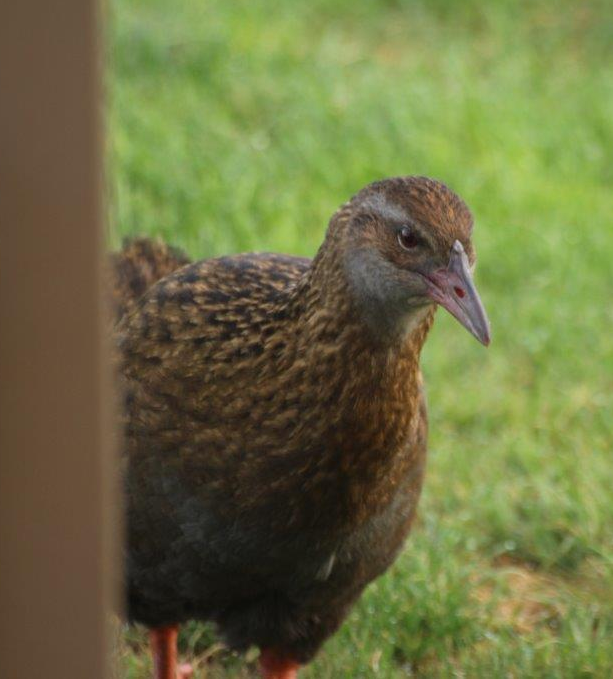
\includegraphics[width=2cm]{weka.png}
}
\graphicspath{ {images/} }

\newcommand{\Lagr}{\mathscr{L}}
\pagestyle{plain}

\title{Introduction into General Relativity\\Assignment 3\\Problem 2}
\author{Simon Crase}

\begin{document}

\maketitle
\thispagestyle{fancy}

\begin{abstract}
Ran out of time.
\end{abstract}


 

\section{$S_M = \int d^4x \, \sqrt{|g|} \, \left[\frac12 \, g^{\mu\nu} \, \partial_\mu \phi \, \partial_\nu \phi - V(\phi)\right]$}
\subsection{Variation}
\begin{align*}
\delta_{\phi} S_M =& \delta_{\phi} \int d^4x \, \sqrt{|g|} \, \left[\frac{1}{2} \, g^{\mu\nu} \, \partial_\mu \phi \, \partial_\nu \phi - V(\phi)\right]\\
=&  \int d^4x \, \sqrt{|g|} \, \left[ \, g^{\mu\nu} \, \partial_\mu \phi \, \partial_\nu \delta \phi - V'(\phi) \delta_{\phi} \right]\\
=& \int d^4x \big[ -\partial_\nu \big(\sqrt{|g|} g^{\mu\nu} \partial_\mu \phi\big) - \sqrt{(|g|)} V'(\phi)\big] \text{, why?}
\end{align*}
\subsection{Equations of motion}
\begin{align*}
-\partial_\nu \big(\sqrt{|g|} g^{\mu\nu} \partial_\mu \phi\big) - \sqrt{(|g|)} V'(\phi)=&0\\
\frac{1}{\sqrt{(|g|)}} \partial_\nu \big(\sqrt{|g|} g^{\mu\nu} \partial_\mu \phi\big) =& -  V'(\phi)
\end{align*}
\subsection{Stress Tensor} \label{subseq:StressTensor}
From (\ref{eq:a}) and Lecture Notes \cite[Lecture III, Section 3]{akhmedev2016}:
\begin{equation}
S_M = \int d^4x \, \sqrt{|g|} \underbrace{\left[\frac12 \, g^{\mu\nu} \, \partial_\mu \phi \, \partial_\nu \phi - V(\phi)\right]}_{\text{Lagrangian}\overset{\Delta}{=}\Lagr}
\end{equation}
So $\Lagr$ is given by
\begin{equation}
\Lagr=\frac12 \, g^{\mu\nu} \, \partial_\mu \phi \, \partial_\nu \phi - V(\phi)
\end{equation}
From the Lecture Notes \cite[(64)]{akhmedev2016}:
\begin{align}
T_{\mu\nu}&\overset{\Delta}{=}2 \frac{\partial \Lagr}{\partial g^{\mu\nu}} - \Lagr g_{\mu\nu} \nonumber \\
&=\frac{\partial [g^{\sigma\tau}\partial_\sigma \phi \partial_\tau \phi]}{\partial g^{\mu\nu}}-[\frac12 \, g^{\sigma\tau} \, \partial_\sigma \phi \, \partial_\tau \phi - V(\phi)] g_{\mu\nu} \nonumber \\
&=\frac{\partial g^{\sigma\tau}}{\partial g^{\mu\nu}}\partial_\sigma \phi \partial_\tau \phi-[\frac12 \, g^{\sigma\tau} \, \partial_\sigma \phi \, \partial_\tau \phi - V(\phi)] g_{\mu\nu} \nonumber \\
&=\partial_\mu \phi \partial_\nu \phi - \frac12 \, g^{\sigma\tau} \, \partial_\sigma \phi \, \partial_\tau \phi + V(\phi) g_{\mu\nu} 
\end{align}

\section{$S_M = \int d^4x \sqrt{|g|} \, F_{\mu\nu}\, F_{\alpha\beta} \, g^{\mu\alpha} \, g^{\nu\beta}.$}
\subsection{Variation}
\begin{align*}
\delta_A S_M =& \delta_A \int d^4x \sqrt{|g|} \, F_{\mu\nu}\, F_{\alpha\beta} \, g^{\mu\alpha} \, g^{\nu\beta} \\
=& 2 \int d^4x \sqrt{|g|} \, F_{\mu\nu} \, g^{\mu\alpha} \, g^{\nu\beta} \, \delta_A F_{\alpha\beta}\\
=& 2 \int d^4x \sqrt{|g|} \, F_{\mu\nu} \, g^{\mu\alpha} \, g^{\nu\beta} \, \delta_A \big(\partial_\alpha A_\beta - \partial_\beta A_\alpha\big)\\
=& 4 \int d^4x \sqrt{|g|} \, F_{\mu\nu} \, g^{\mu\alpha} \, g^{\nu\beta} \, \delta \big(\partial_\alpha A_\beta \big)\\
=& -4 \int d^4x \partial_\alpha \big(\sqrt{|g|} \, F_{\mu\nu} \, g^{\mu\alpha} \, g^{\nu\beta} \,\big) \delta A_\beta\\
=& -4 \int d^4x \partial_\alpha \big(\sqrt{|g|} \, F^{\alpha\beta}  \,\big) \delta A_\beta
\end{align*}
\subsection{Equations of motion}
\begin{align*}
\partial_\alpha \big(\sqrt{|g|} \, F_{\mu\nu} \, g^{\mu\alpha} \, g^{\nu\beta} \,\big) &= 0\\
 D_\alpha F^{\alpha\beta} &= 0
\end{align*}
\subsection{Stress Tensor}
By the same argument as in Section \ref{subseq:StressTensor}:
\begin{equation}
\Lagr= F_{\mu\nu}\, F_{\alpha\beta} \, g^{\mu\alpha} \, g^{\nu\beta}.
\label {eq:a}
\end{equation}

and
\begin{align}
T_{\mu\nu}&\overset{\Delta}{=}2 \frac{\partial \Lagr}{\partial g^{\mu\nu}} - \Lagr g_{\mu\nu}\\
&=2\frac{\partial F_{\sigma\tau}\, F_{\alpha\beta} \, g^{\sigma\alpha} \, g^{\tau\beta}}{\partial g^{\mu\nu}} - F_{\sigma\tau}\, F_{\alpha\beta} \, g^{\sigma\alpha} \, g^{\tau\beta} g_{\mu\nu}
\end{align}
We want:
$$T_{\mu\nu} = 4\big[F_{\mu\alpha} F^\alpha_\nu - \frac{1}{4}g_{\mu\nu} F_{\alpha\beta} F^{\alpha\beta}\big]$$

\begin{thebibliography}{9}

\bibitem{akhmedev2016}
Emil T. Akhmedev,
\emph{Lectures on General Theory of Relativity},
2016,
\url{https://arxiv.org/pdf/1601.04996v6.pdf}.

\end{thebibliography}

\end{document}
